\documentclass[12pt]{article}

\usepackage{listings}

%Adding Image
\usepackage{graphicx}
\graphicspath{{images/}}

%HyperLinks for Table of Contents
\usepackage{hyperref}
\hypersetup{colorlinks = true, citecolor = blue, linkcolor = blue, urlcolor = blue}

%Title
\title{C Language Test 1 }
\author{Sai Krishna Dasari\\Group 7}

%Starting of the Document
\begin{document}
\maketitle %Title will go over here
\pagebreak
\tableofcontents %for making table of contents
\clearpage
\section{Question-1}

\emph{\textbf{Write a program that declares a pointer to an integer and passes it to a function. The function should increment the value of the integer using the pointer, and the program should print the updated value.}}


\subsection{Code}
\begin{lstlisting}[language=C]  
	#include<stdio.h>
	int *ptr , a;
	void increment(int i);
	
	int main()
	{
	  printf("Enter the value of a = ");
	  scanf("%d",&a);
	  ptr = &a ; //Assigning the address to pointer
	  increment(*ptr); //Dereferencing the pointer
	  return 0;
	}
	
	void increment(int i)
	{
  	  *ptr = i + 1 ; //incrementing the value 'a'
  	  printf("Value of Incremented a = %d",*ptr);
	}

\end{lstlisting}

\subsection{Inputs and Output}


	\begin{center}

	Enter the value of \textbf{a = 20}
  

    Value of Incremented \textbf{a = 21}[Fig: \ref{fig_input_output}]

	\end{center}
\pagebreak
\begin{figure}[h]
\centering
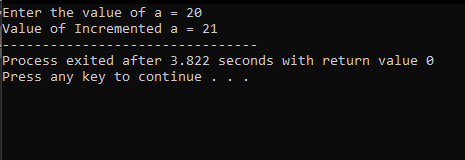
\includegraphics[scale=1.2]{input1.png}
\caption{Input and Output }
\label{fig_input_output}
\end{figure}

\section{Question-2}

\emph{\textbf{Write a program that implements the merge sort algorithm for an array of integers using pointers.}}


\subsection{Code}
\begin{lstlisting}[language=C]

#include <stdio.h>

void merge(int *arr, int left, int mid, int right) {
    int i = left, j = mid + 1, k = 0;
    int temp[right - left + 1];

    while (i <= mid && j <= right) 
	{
        if (*(arr + i) <= *(arr + j))
            temp[k++] = *(arr + i++);
        else
            temp[k++] = *(arr + j++);
    }

    while (i <= mid)
    {
        temp[k++] = *(arr + i++);
	}

    while (j <= right)
    {
        temp[k++] = *(arr + j++);
    }

    for (i = left, k = 0; i <= right; i++, k++)
	{
        *(arr + i) = temp[k];
	}
}

void merge_sort(int *arr, int left, int right) 
{
    if (left >= right)
        return;

    int mid = (left + right) / 2;
    merge_sort(arr, left, mid);
    merge_sort(arr, mid + 1, right);
    merge(arr, left, mid, right);
}

int main() 
{
    int arr[] = {10, 7, 3, 8, 9, 1, 5};
    
    int n = sizeof(arr) / sizeof(arr[0]);
    
    printf("value of n = %d\n",n);

    printf("Unsorted array: ");
    
    for (int i = 0; i < n; i++)
    {
        printf("%d ", *(arr + i));
	}
    printf("\n");

    merge_sort(arr, 0, n - 1);

    printf("Sorted array: ");
    for (int i = 0; i < n; i++)
    {
        printf("%d ", *(arr + i));
    }
    printf("\n");

    return 0;
}

\end{lstlisting}

\subsection{Inputs and Output}
\begin{center}
Value of n = 7\\
Unsorted array: 10 7 3 8 9 1 5\\
Sorted array: 1 3 5 7 8 9 10[Fig: \ref{fig_input_output}]\\
\end{center}
\begin{figure}[h]
\centering
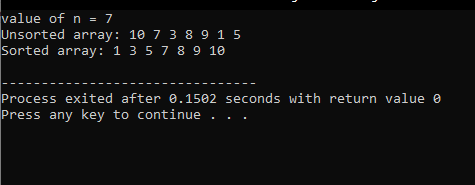
\includegraphics[scale=0.8]{input2.png}
\caption{Input and Output}
\label{fig_input_output}
\end{figure}

\end{document}